% vim: set spell spelllang=en tw=100 et sw=4 sts=4 :

\documentclass[a0paper]{tikzposter}

\usepackage{algorithm2e,algpseudocode}
\usepackage{complexity}
\usepackage{wrapfig}
\usepackage{microtype}
\usepackage{gnuplot-lua-tikz}
\usepackage{amssymb}
\usepackage{amsmath}
\usepackage{sfmath}

\usepackage{lmodern}
\renewcommand*\familydefault{\sfdefault}
\usepackage[T1]{fontenc}

\newcommand{\McSplit}{\textproc{McSplit}}

\title{A Partitioning Algorithm for Maximum Common Subgraph Problems}
\author{Ciaran McCreesh, Patrick Prosser and James Trimble}
\institute{University of Glasgow, Glasgow, Scotland}
\titlegraphic{
\includegraphics[keepaspectratio=true,scale=3.5]{UoG_keyline.pdf}}

\settitle{
    \begin{tikzpicture}
        \node (T) [inner sep=0pt] {\begin{minipage}{\linewidth}
                \color{titlefgcolor}
                {\bfseries \Huge \hspace*{10mm}A Partitioning Algorithm for Maximum \\
                \hspace*{10mm}Common Subgraph Problems \par}
                \vspace*{1em}
                {\Large {\bfseries \hspace{10mm}\@author}, \@institute}
        \end{minipage}};

        \node at (T.east) [anchor=center, inner sep=0pt, xshift=-12cm] {\@titlegraphic};
    \end{tikzpicture}
}

% University of Glasgow standard colours
\definecolor{uofguniversityblue}{rgb}{0, 0.219608, 0.396078}

\definecolor{uofgheather}{rgb}{0.356863, 0.32549, 0.490196}
\definecolor{uofgaquamarine}{rgb}{0.603922, 0.72549, 0.678431}
\definecolor{uofgslate}{rgb}{0.309804, 0.34902, 0.380392}
\definecolor{uofgrose}{rgb}{0.823529, 0.470588, 0.709804}
\definecolor{uofgmocha}{rgb}{0.709804, 0.564706, 0.47451}

\definecolor{uofglawn}{rgb}{0.517647, 0.741176, 0}
\definecolor{uofgcobalt}{rgb}{0, 0.615686, 0.92549}
\definecolor{uofgturquoise}{rgb}{0, 0.709804, 0.819608}
\definecolor{uofgsunshine}{rgb}{1.0, 0.862745, 0.211765}
\definecolor{uofgpumpkin}{rgb}{1.0, 0.72549, 0.282353}
\definecolor{uofgthistle}{rgb}{0.584314, 0.070588, 0.447059}
\definecolor{uofgpillarbox}{rgb}{0.701961, 0.047059, 0}
\definecolor{uofglavendar}{rgb}{0.356863, 0.301961, 0.580392}

\definecolor{uofgsandstone}{rgb}{0.321569, 0.278431, 0.231373}
\definecolor{uofgforest}{rgb}{0, 0.317647, 0.2}
\definecolor{uofgburgundy}{rgb}{0.490196, 0.133333, 0.223529}
\definecolor{uofgrust}{rgb}{0.603922, 0.227451, 0.023529}

\definecolorstyle{UofG}{
}{
    % Background Colors
    \colorlet{backgroundcolor}{uofgsandstone!80!white}
    \colorlet{framecolor}{black}
    % Title Colors
    \colorlet{titlefgcolor}{white}
    \colorlet{titlebgcolor}{uofguniversityblue}
    % Block Colors
    \colorlet{blocktitlebgcolor}{white}
    \colorlet{blocktitlefgcolor}{uofguniversityblue}
    \colorlet{blockbodybgcolor}{white}
    \colorlet{blockbodyfgcolor}{black}
    % Innerblock Colors
    \colorlet{innerblocktitlebgcolor}{uofguniversityblue}
    \colorlet{innerblocktitlefgcolor}{black}
    \colorlet{innerblockbodybgcolor}{uofgsandstone}
    \colorlet{innerblockbodyfgcolor}{black}
    % Note colors
    \colorlet{notefgcolor}{black}
    \colorlet{notebgcolor}{uofgrust}
    \colorlet{noteframecolor}{red}
}

\usetheme{Autumn}
\usecolorstyle{UofG}

\tikzposterlatexaffectionproofoff

\useblockstyle[bodyverticalshift=-1cm, roundedcorners=0]{Default}

\renewcommand{\Huge}{\fontsize{77.2}{96}\selectfont}

% Styles for drawings

\tikzset{edge/.style={line width=3pt, color=uofgsandstone}}
\tikzset{ledge/.style={line width=3pt, color=uofgsandstone!40!white}}
\tikzset{hedge/.style={line width=3pt, color=uofgsandstone, dashed}}

\setlength\intextsep{0pt}

\begin{document}
\maketitle

\begin{columns}
\column{1}
{
    \colorlet{blockbodybgcolor}{uofgcobalt}
    \colorlet{blocktitlebgcolor}{uofgcobalt}
    \block[bodyverticalshift=0.5cm, bodyinnersep=3mm]{}{
        \centering\begin{minipage}{0.94\textwidth}
            \Large We introduce a new \textbf{branch and bound} algorithm for the \textbf{maximum common
            subgraph} and \textbf{maximum common connected subgraph} problems which is based
            around vertex labelling and partitioning. Our method resembles
            a constraint programming approach, but uses a novel compact
            domain store to reduce
            the memory and computation requirements.  Experiments
            show a \textbf{speedup of more than an order of magnitude} over the state of the
            art, and demonstrate that we can operate on \textbf{much larger graphs} without
            running out of memory.
%            We show how to generate \textbf{really hard} random instances for \textbf{subgraph
%            isomorphism} problems. For the non-induced variant, we predict and observe a phase
%            transition between satisfiable and unsatisfiable instances, with a corresponding
%            complexity peak seen in \textbf{three different solvers}. For the induced variant, much
%            richer behaviour is observed, and \textbf{constrainedness} gives a better measure of
%            difficulty than does proximity to a phase transition. We also discuss \textbf{variable
%            and value ordering} heuristics, and their relationship to the \textbf{expected number of
%            solutions}.
        \end{minipage}
        \vspace*{0.4cm}
    }
}
\end{columns}

\begin{columns}
\column{0.5}

\block{The Maximum Common Subgraph Problem}{
\begin{wrapfigure}[7]{r}{0.47\linewidth}
    \begin{flushright}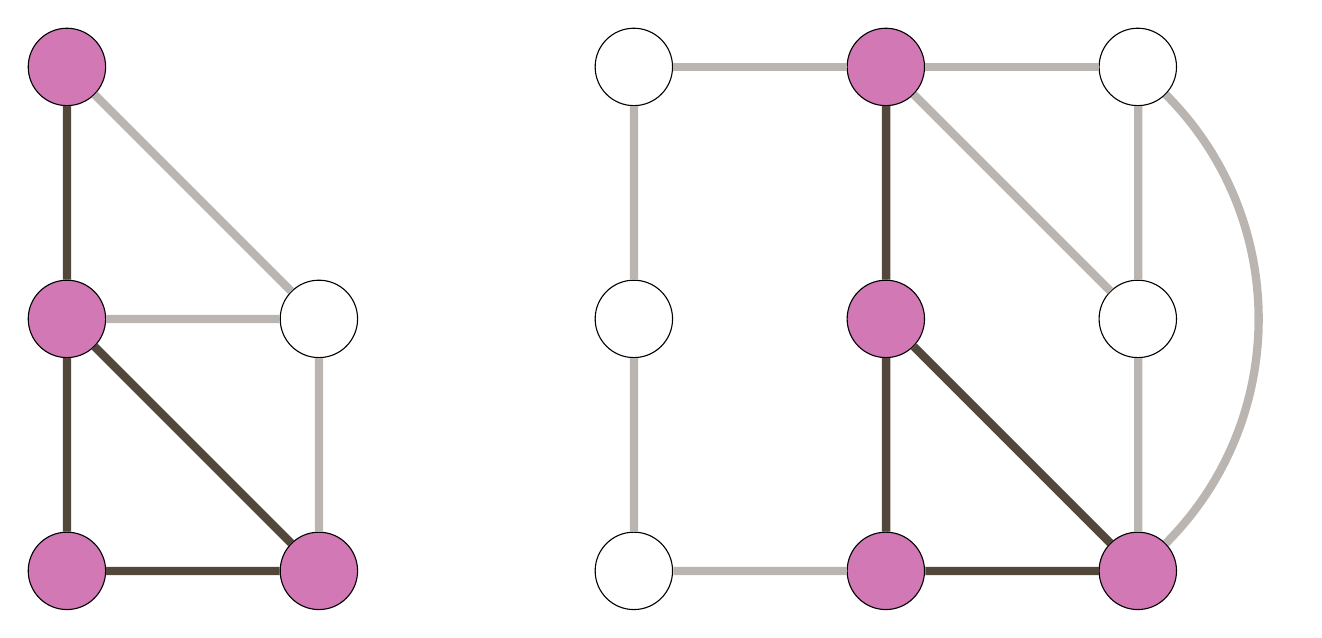
\begin{tikzpicture}[scale=1.6]%{{{
        \node[draw, circle, fill=uofgrose, inner sep=8pt, font=\bfseries] (Na) at (1,  0)
        {\vphantom{0}};
        \node[draw, circle, fill=uofgrose, inner sep=8pt, font=\bfseries] (Nb) at (1, -2)
        {\vphantom{0}};
        \node[draw, circle, fill=uofgrose, inner sep=8pt, font=\bfseries] (Nc) at (1, -4)
        {\vphantom{0}};
        \node[draw, circle, fill=uofgrose, inner sep=8pt, font=\bfseries] (Nd) at (3, -4)
        {\vphantom{0}};
        \node[draw, circle, fill=white, inner sep=8pt, font=\bfseries] (Ne) at (3, -2)
        {\vphantom{0}};

        \draw [edge] (Na) -- (Nb);
        \draw [edge] (Nb) -- (Nc);
        \draw [edge] (Nc) -- (Nd);
        \draw [edge] (Nb) -- (Nd);
        \draw [ledge] (Na) -- (Ne);
        \draw [ledge] (Nb) -- (Ne);
        \draw [ledge] (Nd) -- (Ne);

        \node[draw, circle, fill=uofgrose, inner sep=8pt, font=\bfseries] (N1) at (7.5,  0) {\vphantom{0}};
        \node[draw, circle, fill=white, inner sep=8pt, font=\bfseries] (N2) at (9.5,  0) {\vphantom{0}};
        \node[draw, circle, fill=uofgrose, inner sep=8pt, font=\bfseries] (N3) at (7.5, -2) {\vphantom{0}};
        \node[draw, circle, fill=white, inner sep=8pt, font=\bfseries] (N4) at (9.5, -2) {\vphantom{0}};
        \node[draw, circle, fill=uofgrose, inner sep=8pt, font=\bfseries] (N5) at (7.5, -4) {\vphantom{0}};
        \node[draw, circle, fill=uofgrose, inner sep=8pt, font=\bfseries] (N6) at (9.5, -4) {\vphantom{0}};
        \node[draw, circle, fill=white, inner sep=8pt, font=\bfseries] (N7) at (5.5,  0) {\vphantom{0}};
        \node[draw, circle, fill=white, inner sep=8pt, font=\bfseries] (N8) at (5.5, -2) {\vphantom{0}};
        \node[draw, circle, fill=white, inner sep=8pt, font=\bfseries] (N9) at (5.5, -4) {\vphantom{0}};

        \draw [ledge] (N1) -- (N2);
        \draw [edge] (N1) -- (N3);
        \draw [ledge] (N1) -- (N4);
        \draw [ledge] (N2) -- (N4);
        \draw [edge] (N3) -- (N5);
        \draw [edge] (N3) -- (N6);
        \draw [ledge] (N4) -- (N6);
        \draw [edge] (N5) -- (N6);
        \draw [ledge] (N2) to [in=45, out=315] (N6);
        \draw [ledge] (N1) -- (N7);
        \draw [ledge] (N5) -- (N9);
        \draw [ledge] (N7) -- (N8);
        \draw [ledge] (N8) -- (N9);
    \end{tikzpicture}\end{flushright}

\end{wrapfigure}

The \textbf{maximum common subgraph} family of problems involves finding a large
graph that appears in each of two input graphs.
Such problems have arisen in molecular science---where graphs often represent
molecules---malware detection, source code analysis, and computer vision.

\bigskip

    Maximum common subgraph problems are \mbox{NP-hard}, and remain challenging
computationally. Recent practical progress has been made by using constraint
programming and
mathematical programming, by reducing
to the maximum clique problem, and by
adapting subgraph isomorphism algorithms. Some
special cases also have practical polynomial time algorithms.

\bigskip

We consider the \textbf{maximum common induced subgraph} problem, in
which the objective is to find a graph with as many vertices as possible which
is an induced subgraph of each of two input graphs.  The diagram shows a simple instance
with an optimal solution highlighted.
}

\block{The \McSplit\ Algorithm}{

We introduce a branch and bound algorithm which exploits special properties of the
problem to allow a much faster exploration of the search space, whilst
retaining the filtering and bounding benefits of a constraint programming
approach. 

\bigskip

Using depth-first search, the \McSplit\ algorithm builds up an injective mapping from a subset
of vertices in the pattern graph to a subset of vertices in the target graph.  
Remaining vertices are partitioned into \textbf{label classes} according to the set of mapped
vertices to which they are adjacent; each pattern-graph vertex may only be mapped to target-graph
vertices in the same label class.  We thus avoid
the need for a conventional domain store in which the possible mappings for each
vertex are stored explicitly.  
}

\block{The Relationship to Constraint Programming}{

    \bigskip

    Our experimental results suggest that \McSplit\ has broadly
    similar performance trends to the constraint programming,
    forward-checking (CP-FC) algorithm of Ndiaye and Solnon
    (2011), but with much lower constant factors and memory
    usage.  In the figure below, we plot the number
    of recursive calls made by our algorithm versus the number
    made by CP-FC, for unlabelled, unconnected
    problem instances. (Rather than a simple scatter plot,
    darker colours are used to indicate a higher density of points around
    a location.) We see a close correlation: \McSplit\ typically
    does slightly less work, and sometimes does more, but instances with
    more than one order of magnitude difference in
    search tree size are rare.

    Why is this?  The key
    observation is that \McSplit\ may be considered to be a different version of the CP-FC algorithm,
    using an unconventional domain store and more efficient filtering algorithms.
    This is possible because in the CP model, \textbf{any two domains are either identical
    or disjoint}, excluding $\bot$.  We explore this relationship further in the paper.

    \vspace*{1em}

\begin{center}
    \small\input{gen-graph-plain-james-versus-cp-fc-nodes-scatter}
\end{center}
}

\block{See the Paper For\ldots}{
    \begin{itemize}
        \item ~ How to extend the algorithm to handle vertex and edge labels
        \item ~ Additional experimental results
    \end{itemize}
}

\column{0.5}

\block{Experiments}{
We compare our implementation of \McSplit\ against the best existing constraint
programming implementations, clique encodings, and the
$k{\downarrow}$ algorithm of McCreesh et al. (2017).  Each of these comparator
programs is an optimised, dedicated implementation and does not use a
general-purpose constraint programming toolkit.

\bigskip

For the unlabelled problem, we used 4,100 instances from a
database of randomly-generated maximum common subgraph instances.  For
the labelled variant, we used 8,140 instances from the same database.  \McSplit\ is
more than an order of magnitude faster than its nearest competitor on unlabelled instances.
On labelled instances, the clique encoding remains the single best solver.

    \vspace*{2em}

    \begin{center}
        \small
        \input{gen-graph-plain-cumulative}
    \end{center}

    \vspace*{2em}

    \begin{center}
        \small
        \input{gen-graph-33ved-cumulative}
    \end{center}

    \vspace*{2em}

We also ran the algorithms on a set of 5,725 larger instances used in recent
studies of subgraph isomorphism and maximum common subgraph; a modified version
of \McSplit\ is the single best solver on this set of instances.

    \vspace*{2em}

    \begin{center}
        \small
        \input{gen-graph-sip-cumulative}
    \end{center}
}

\end{columns}

%\begin{columns}
%\column{0.5}
%
%\column{0.5}
%
%%\block{Future Work}{
%%    \begin{itemize}
%%        \item ~ Branching on vertices in both graphs
%%        \item ~ Applying the partitioning data structure to other problems
%%    \end{itemize}
%%    \vspace*{0.25em}
%%}
%
%\end{columns}

{
    \colorlet{blockbodybgcolor}{uofgsandstone!80!white}
    \colorlet{blocktitlebgcolor}{uofgsandstone!80!white}
    \block[bodyverticalshift=-0.5cm]{}{
        This work was supported by the Engineering and Physical Sciences Research Council [grant numbers EP/K503058/1 and
        EP/M508056/1]. \hfill \texttt{\textcolor{white}{j.trimble.1@research.gla.ac.uk}}
    }
}

\end{document}

